\documentclass[10pt,landscape,a4paper]{article}
%\usepackage[utf8]{inputenc}
%\usepackage[ngerman]{babel}
\usepackage[normalem]{ulem}
\usepackage{tikz}
\usetikzlibrary{shapes,positioning,arrows,fit,calc,graphs,graphs.standard}
\usepackage[nosf]{kpfonts}
\usepackage[t1]{sourcesanspro}
%\usepackage[lf]{MyriadPro}
%\usepackage[lf,minionint]{MinionPro}
\usepackage{multicol}
\usepackage{wrapfig}
\usepackage[top=0mm,bottom=1mm,left=0mm,right=1mm]{geometry}
\usepackage[framemethod=tikz]{mdframed}
\usepackage{microtype}
%\usepackage{physics}
\usepackage{tabularx}
\usepackage{hhline}
\usepackage{makecell}
\usepackage{mathtools}

\usepackage{listings}

\DeclarePairedDelimiter{\ceil}{\lceil}{\rceil}

\newcommand\codeblue[1]{\textcolor{blue}{\code{#1}}}

\usepackage{lastpage}
\usepackage{datetime}
\yyyymmdddate
\renewcommand{\dateseparator}{-}
\let\bar\overline

\definecolor{myblue}{cmyk}{1,.72,0,.38}

\def\firstcircle{(0,0) circle (1.5cm)}
\def\secondcircle{(0:2cm) circle (1.5cm)}

\colorlet{circle edge}{myblue}
\colorlet{circle area}{myblue!5}

\tikzset{filled/.style={fill=circle area, draw=circle edge, thick},
outline/.style={draw=circle edge, thick}}

\pgfdeclarelayer{background}
\pgfsetlayers{background,main}

%\everymath\expandafter{\the\everymath \color{myblue}}
%\everydisplay\expandafter{\the\everydisplay \color{myblue}}


\renewcommand{\baselinestretch}{.8}
\pagestyle{empty}

\global\mdfdefinestyle{header}{%
  linecolor=gray,linewidth=1pt,%
  leftmargin=0mm,rightmargin=0mm,skipbelow=0mm,skipabove=0mm,
}

\newcommand{\header}{
  \begin{mdframed}[style=header]
    \footnotesize
    \sffamily
    ACC1701XA Midterms Cheatsheet v1.1 (\today)\\
    by~Your Name,~page~\thepage~of~\pageref{LastPage}
  \end{mdframed}
}

\let\counterwithout\relax
\let\counterwithin\relax
\usepackage{chngcntr}

\usepackage{verbatim}

\usepackage{etoolbox}
\makeatletter
\preto{\@verbatim}{\topsep=0pt \partopsep=0pt }
\makeatother

\counterwithin*{equation}{section}
\counterwithin*{equation}{subsection}
\usepackage{enumitem}
\newlist{legal}{enumerate}{10}
\setlist[legal]{label*=\arabic*.,leftmargin=2.5mm}
\setlist[itemize]{leftmargin=3mm}
\setlist[enumerate]{leftmargin=3.5mm}
\setlist{nosep}
\usepackage{minted}

\def\code#1{\texttt{#1}}

\newenvironment{descitemize} % a mixture of description and itemize
{\begin{description}[leftmargin=*,before=\let\makelabel\descitemlabel]}
{\end{description}}

\newcommand{\descitemlabel}[1]{%
  \textbullet\ \textbf{#1}%
}
\makeatletter



\renewcommand{\section}{\@startsection{section}{1}{0mm}%
  {.2ex}%
  {.2ex}%x
{\color{myblue}\sffamily\small\bfseries}}
\renewcommand{\subsection}{\@startsection{subsection}{1}{0mm}%
  {.2ex}%
  {.2ex}%x
{\sffamily\bfseries}}
\renewcommand{\subsubsection}{\@startsection{subsubsection}{1}{0mm}%
  {.2ex}%
  {.2ex}%x
{\rmfamily\bfseries}}

\global\let\tikz@ensure@dollar@catcode=\relax

\def\mathcolor#1#{\@mathcolor{#1}}
\def\@mathcolor#1#2#3{%
  \protect\leavevmode
  \begingroup
  \color#1{#2}#3%
  \endgroup
}

\makeatother
\setlength{\parindent}{0pt}

\setminted{tabsize=2, breaklines}
% Remove belowskip of minted
\setlength\partopsep{-\topsep}

\newcolumntype{a}{>{\hsize=1.5\hsize}X}
% \newcolumntype{b}{>{\hsize=.25\hsize}X}

\setlength\columnsep{1.5pt}
\setlength\columnseprule{0.1pt}

\begin{document}
\setlength{\abovedisplayskip}{0pt}
\setlength{\belowdisplayskip}{0pt}

% \header

\scriptsize
\begin{multicols*}{4}
  \raggedcolumns

  \section{Accounting in Business \& FS Overview}
  \subsection{International Accounting Standards Board (IASB)}
  \subsubsection{}
  \begin{itemize}
    \item Qualitative Characteristics: Relevance, Faithful Representation,
    \item Comparability, Veriiability, Timeliness, Understandability
    \item IASB -> IFRS -> FRS (Singapore)
    \item Overall ethical conduct
  \end{itemize}
  \subsubsection{Auditors \& External Audit}
  \begin{itemize}
    \item Independent certified public accountant (CPA) perform external audits.
    \item Provides public with assurance that FSs are not misleading.
  \end{itemize}
  \subsection{The Accounting Equation}
  \begin{itemize}
    \item Assets = Liabilities + Equity
    \item = Liabilities + Share Capital + Retained Earnings
    \item = Liabilities + Share Capital + Revenue - Expenses - Dividends
  \end{itemize}
  \subsubsection{Asset}
  \begin{itemize}
    \item A \textbf{present resource}
    \item Due to a \textbf{past event}
    \item That will \textbf{result in future benefits}
  \end{itemize}
  \subsubsection{Liabilitity}
  \begin{itemize}
    \item An \textbf{obligation}
    \item Due to a \textbf{past event}
    \item That will \textbf{result in future outflow} of resources upon \textbf{settlement}
  \end{itemize}
  \subsubsection{Equity}
  \begin{itemize}
    \item Owner's claim on the residual interest after deducting all Liabilities
    \item net assets (total assets - total liabilities)
  \end{itemize}
  \subsubsection{Claims}
  \begin{itemize}
    \item Share Capital / Capital Stock: contributed by owners
    \item Retained earnings: equity earned by company
  \end{itemize}
  \subsection{IASB Definitions}
  \begin{itemize}
    \item Income: inflow/enhancement of assets (OR decrease in liabilities -> equity up). During accounting period, not by contributions from owners.
    \item Expense: outflow/depletions of assets (OR incurrance of liability -> equity down). During accouting period.
    \item Capital Maintenance Adjustments: Revaulation of assets/liabilities. \textbf{not included in income statement}. Treated as Other Comprehensive Income (OCI)
  \end{itemize}
  \subsection{The Financial Statements}
  \subsubsection{Statement of Financial Position AKA Balance Sheet (SFP/BS)}
  \begin{itemize}
    \item A = L + E
    \item A snapshot of company's economic resources and obligations
    \item Limitation: Assets recorded at cost, not market value. Usually book v < market v
  \end{itemize}
  \subsubsection{Statement of Comprehensive Income (SCI)}
  \begin{itemize}
    \item Rev - Exp = Net Income (NI)
    \item NI + OCI = Comprehensive Income 
    \item Revenues: Operation earnings, Net Income: NI = Rev - Exp, Other Comprehensive Income: investments etc.
    \item Shows economic performance over time.
    \item Either Income statement \& SCI together or not. OCI can be seperate (IAS1)
  \end{itemize}
  \subsubsection{Statement of Changes in Equity (SCE)}
  \begin{itemize}
    \item Beginning Equity + Net change in Capital + Net Income - Dividends + OCI = End Equity
  \end{itemize}
  \subsubsection{Statement of Cash Flows (SCF)}
  \begin{itemize}
    \item CFO + CFI + CFF (operating, Investing, financing)
    \item CFO: revenue, etc. CFI: buying equipment, land, etc. CFF: investors investing, paying dividends etc.
  \end{itemize}
  \subsection{Relationships among the 4 FSs}
  \begin{tabular}{l}
    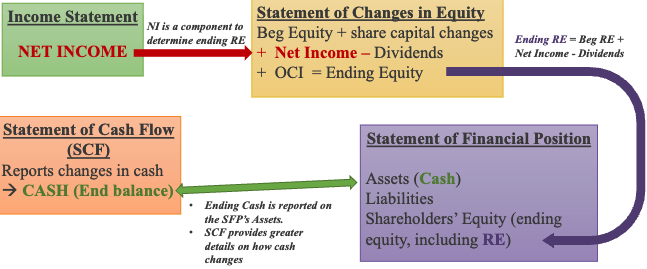
\includegraphics[width=0.95\linewidth]{relationship-of-fs}
  \end{tabular}
  \subsection{Fundamental Concepts \& Assumptions of Accounting}
  \begin{itemize}
    \item Separate entity concept: Activity of a bz is separate from its owners
    \item Time-period assumption: bz's activities can be divided into time periods (monthly,quarterly,etc)
    \item Assumption of arm's-length transactions
    \item Cost Principle
    \item Fair value Principle
    \item Monetary measurement concept
    \item Going concern assumption
  \end{itemize}
  \section{Mechanics of Accounting}
  \subsection{Credit/Debit}
  \begin{itemize}
    \item Depends on Type of account.
    \item Normal Debit/Normal Credit
  \end{itemize}
  \begin{tabular}{l}
    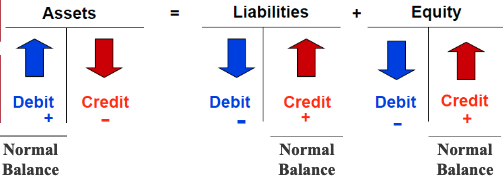
\includegraphics[width=0.6\linewidth]{dr-cr}
  \end{tabular}
  \begin{minipage}{0.3\columnwidth}
    depends on where the account lies on the AE.
  \end{minipage}
  \subsubsection{Subsubheading 2.1.1}
  \begin{itemize}
    \item Point 1
    \item Point 2
  \end{itemize}

  \section{Heading 3}
  \begin{itemize}
    \item Point 1
    \item Point 2
    \item Point 3
  \end{itemize}

  \begin{tabular}{l}
    
\includegraphics[width=0.7\linewidth]{placeholder-image}
  \end{tabular}
  \begin{minipage}{0.15\columnwidth}
    Placeholder note for image
  \end{minipage}

  \subsection{Heading 4}
  \begin{itemize}
    \item Point 1
    \item Point 2
  \end{itemize}

  \subsubsection{Heading 4.1}
  \begin{itemize}
    \item Point 1
    \item Point 2
  \end{itemize}

  \begin{tabularx}{0.4\columnwidth}{X}
    \begin{itemize}
      \item Placeholder tabularx content
    \end{itemize}
  \end{tabularx}

  \begin{minted}{C}
  // Placeholder code block
  int main() {
    return 0;
  }
  \end{minted}

\end{multicols*}
\end{document}
